\section{Ablation Studies}
\label{sec:5_4}

Ablation studies quantify contributions of individual components.

\begin{figure}[htbp]
    \centering
    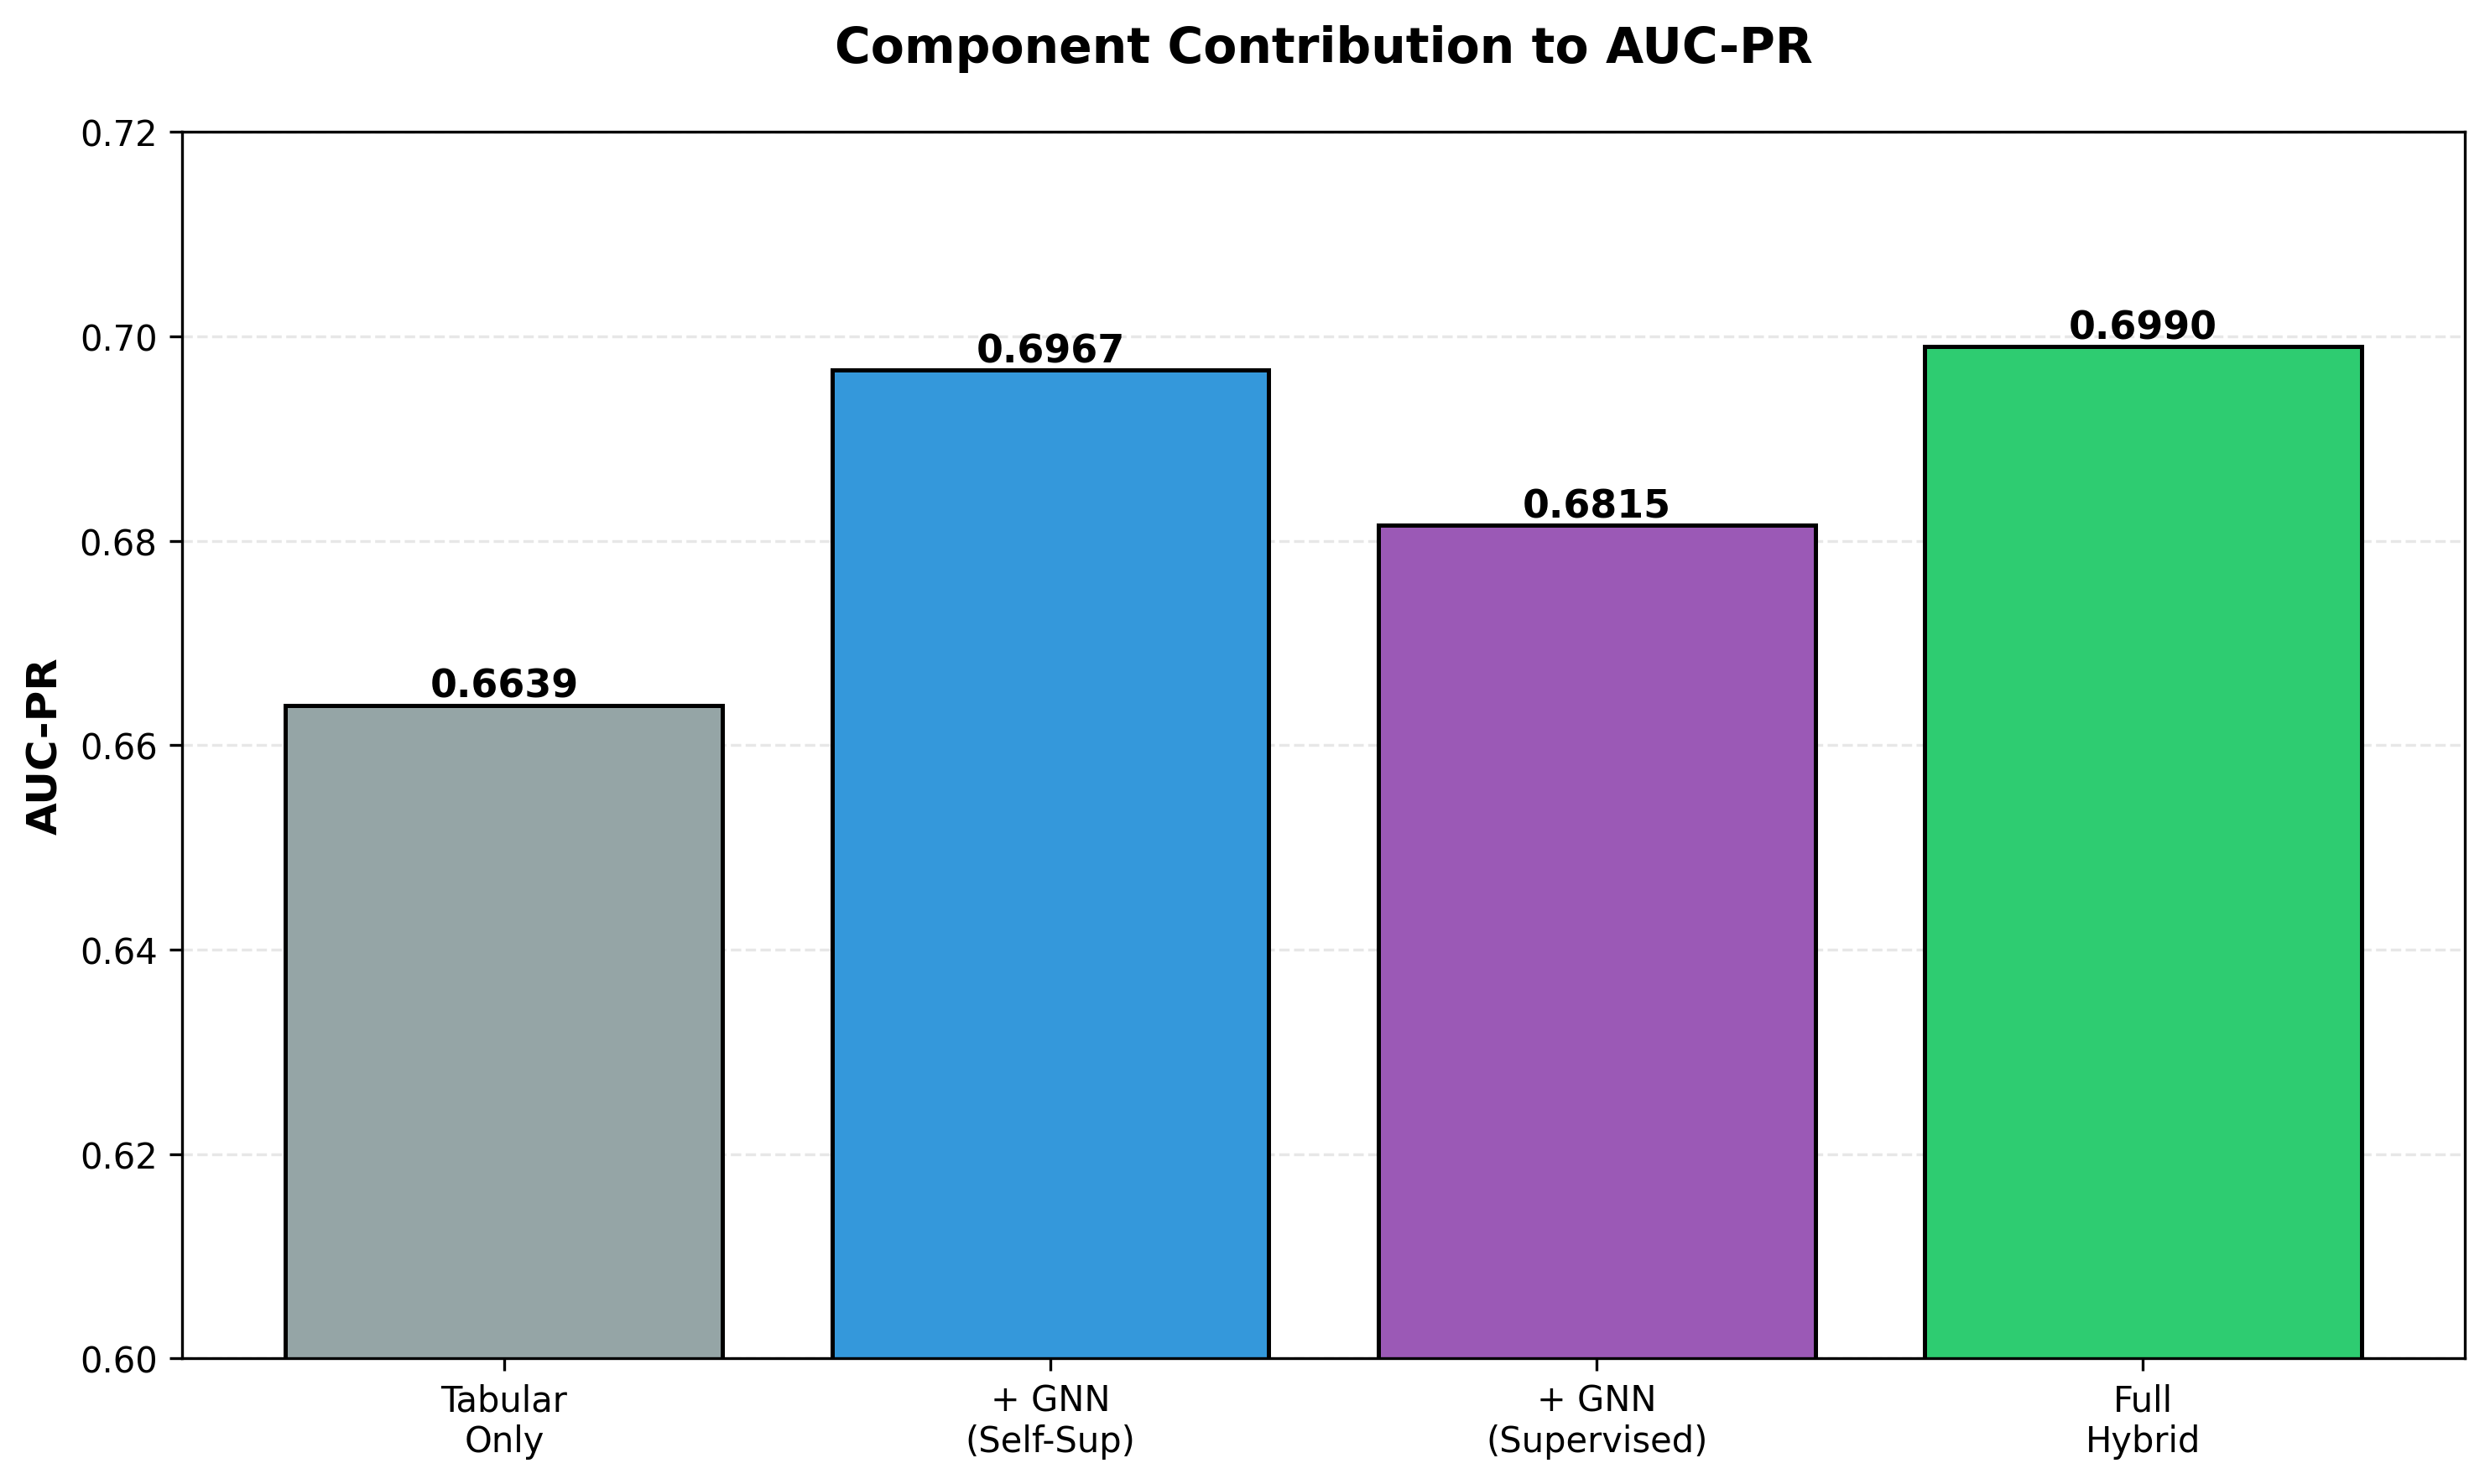
\includegraphics[width=0.8\textwidth]{figures/fig_5_5_4_1.png}
    \caption{Component Contribution to AUC-PR}
    \label{fig:5_4}
\end{figure}

\begin{table}[htbp]
    \centering
    \caption{Supervised vs Self-Supervised GNN}
    \label{tab:5_4}
    \begin{tabular}{lcccc}
        \toprule
        Training Mode & AUC-PR & AUC-ROC & P@0.5 & R@0.5 \\
        \midrule
        Self-Supervised (Link Prediction) & 0.6967 & 0.9426 & 70.6\% & 64.9\% \\
        Supervised (Node Classification) & 0.6815 & 0.9448 & 70.6\% & 65.8\% \\
        \bottomrule
    \end{tabular}
\end{table}

Both training modes perform comparably within run-to-run variance. The supervision signal is helpful but XGBoost can learn from labels regardless of GNN training mode.

\textbf{Feature Group Ablation:}

\begin{table}[htbp]
    \centering
    \caption{Feature Set Ablation}
    \label{tab:5_5}
    \begin{tabular}{lc}
        \toprule
        Feature Set & AUC-PR \\
        \midrule
        Full (65 features + GNN) & 0.6990 \\
        Without SEON Boolean & 0.6521 ($-6.7\%$) \\
        Without SEON Categorical & 0.6342 ($-9.3\%$) \\
        Without Listing Features & 0.6687 ($-4.3\%$) \\
        Without Temporal Features & 0.6891 ($-1.4\%$) \\
        Without GNN Embeddings & 0.6639 ($-5.0\%$) \\
        \bottomrule
    \end{tabular}
\end{table}

SEON categorical features (ip\_country, device\_type) contribute most (+9.3\%), followed by SEON boolean (+6.7\%) and GNN embeddings (+5.0\%). Temporal features show minimal independent contribution.
